% ════════════════════════════════════════════════════════════════════════════
%  ПРЕЗЕНТАЦИЯ К ПРЕДЗАЩИТЕ ВКР
%  Сравнение эффективности нейросетей и классических статистических моделей
%  в прогнозировании курса валют
% ════════════════════════════════════════════════════════════════════════════

\documentclass[12pt, aspectratio=169]{beamer}

% Подключаем общую преамбулу (пакеты, цвета, стили tcolorbox, шапка/подвал)
% ════════════════════════════════════════════════════════════════════════════
%  preamble.tex
%  Преамбула: пакеты, тема, цвета, стили tcolorbox, шапка/подвал.
%  Менять только если нужно изменить ОФОРМЛЕНИЕ. Контент презентации
%  лежит в main.tex (метаданные) и в slides/ (сами слайды).
% ════════════════════════════════════════════════════════════════════════════

% ─── Пакеты ─────────────────────────────────────────────────────────────────
\usepackage[utf8]{inputenc}
\usepackage[T2A]{fontenc}
\usepackage[russian]{babel}
\usepackage{booktabs}
\usepackage{array}
\usepackage{colortbl}
\usepackage{pgfplots}
\pgfplotsset{compat=1.18}
\usepackage{tikz}
\usetikzlibrary{shapes.geometric, arrows.meta, positioning, shadows, fit, calc}
\usepackage{amsmath}
\usepackage{amssymb}
\usepackage{fontawesome5}
\usepackage{multirow}
\usepackage{makecell}
\usepackage{xcolor}
\usepackage{tcolorbox}
\tcbuselibrary{skins, breakable}

% ─── Тема и цветовая схема ──────────────────────────────────────────────────
% TODO (опционально): чтобы поменять «фирменный» цвет всей презентации,
% достаточно изменить RGB у primary / secondary / accent ниже.
\usetheme{Madrid}
\usecolortheme{default}

\definecolor{primary}{RGB}{13, 71, 161}     % основной (синий)
\definecolor{secondary}{RGB}{21, 101, 192}  % вторичный
\definecolor{accent}{RGB}{255, 143, 0}      % акцент (оранжевый)
\definecolor{success}{RGB}{27, 94, 32}      % зелёный (успех)
\definecolor{danger}{RGB}{183, 28, 28}      % красный (предупреждение)
\definecolor{light}{RGB}{227, 242, 253}     % светлый фон блоков
\definecolor{darktext}{RGB}{13, 13, 13}
\definecolor{mygray}{RGB}{96, 125, 139}

\setbeamercolor{palette primary}{bg=primary, fg=white}
\setbeamercolor{palette secondary}{bg=secondary, fg=white}
\setbeamercolor{palette tertiary}{bg=primary!80, fg=white}
\setbeamercolor{palette quaternary}{bg=primary, fg=white}
\setbeamercolor{structure}{fg=primary}
\setbeamercolor{frametitle}{bg=primary, fg=white}
\setbeamercolor{title}{bg=primary, fg=white}
\setbeamercolor{block title}{bg=primary, fg=white}
\setbeamercolor{block body}{bg=light}
\setbeamercolor{block title alerted}{bg=danger, fg=white}
\setbeamercolor{block body alerted}{bg=danger!10}
\setbeamercolor{block title example}{bg=success, fg=white}
\setbeamercolor{block body example}{bg=success!10}
\setbeamercolor{item}{fg=primary}
\setbeamercolor{subitem}{fg=secondary}

\setbeamerfont{title}{size=\Large, series=\bfseries}
\setbeamerfont{frametitle}{size=\large, series=\bfseries}

\setbeamertemplate{navigation symbols}{}

% ─── Подвал слайда ──────────────────────────────────────────────────────────
\setbeamertemplate{footline}{%
  \leavevmode%
  \hbox{%
    \begin{beamercolorbox}[wd=.4\paperwidth,ht=2.5ex,dp=1.125ex,leftskip=.3cm]{palette primary}%
      \usebeamerfont{author in head/foot}\insertshortauthor
    \end{beamercolorbox}%
    \begin{beamercolorbox}[wd=.4\paperwidth,ht=2.5ex,dp=1.125ex,center]{palette secondary}%
      \usebeamerfont{title in head/foot}\insertshorttitle
    \end{beamercolorbox}%
    \begin{beamercolorbox}[wd=.2\paperwidth,ht=2.5ex,dp=1.125ex,rightskip=.3cm,right]{palette primary}%
      \usebeamerfont{date in head/foot}
      \insertframenumber{} / \inserttotalframenumber
    \end{beamercolorbox}%
  }%
}

% ─── Стили цветных «карточек» (tcolorbox) ───────────────────────────────────
% В слайдах используются 4 готовых стиля:
%   infobox    — синяя полоса слева (нейтральная информация)
%   formulabox — оранжевая рамка   (формулы / ключевые определения)
%   warnbox    — красная полоса    (предупреждения, минусы)
%   successbox — зелёная полоса    (плюсы, выводы)
\tcbset{
  infobox/.style={
    enhanced, boxrule=0pt, frame hidden,
    colback=light, left=4pt, right=4pt, top=2pt, bottom=2pt,
    borderline west={3pt}{0pt}{primary}
  },
  formulabox/.style={
    enhanced, boxrule=1pt,
    colframe=accent, colback=accent!10,
    left=4pt, right=4pt, top=2pt, bottom=2pt,
    rounded corners
  },
  warnbox/.style={
    enhanced, boxrule=0pt, frame hidden,
    colback=danger!8, left=4pt, right=4pt, top=2pt, bottom=2pt,
    borderline west={3pt}{0pt}{danger}
  },
  successbox/.style={
    enhanced, boxrule=0pt, frame hidden,
    colback=success!8, left=4pt, right=4pt, top=2pt, bottom=2pt,
    borderline west={3pt}{0pt}{success}
  }
}


% ─── Метаданные презентации ─────────────────────────────────────────────────
\title[Нейросети vs ARIMA]{Сравнение эффективности нейросетей и классических статистических моделей в прогнозировании курса валют}
\subtitle{Выпускная квалификационная работа}
\author[Багаев Эмир]{Багаев Эмир\\[4pt]Группа: МИ-1}
\institute[Вуз]{Ташкентский Государственный Транспортный Университет}
\date{2026}

% ════════════════════════════════════════════════════════════════════════════
\begin{document}
% ════════════════════════════════════════════════════════════════════════════

% ─── Титульный слайд ────────────────────────────────────────────────────────
\begin{frame}[plain]
  \begin{tikzpicture}[remember picture, overlay]
    \fill[primary] (current page.north west) rectangle (current page.south east);
    \fill[accent] (current page.south west) rectangle
      ([yshift=6pt]current page.south east);
    \fill[white, opacity=0.05] ([xshift=-2cm,yshift=-2cm]current page.north east)
      circle (5cm);
    \fill[secondary, opacity=0.3] ([xshift=1cm,yshift=2cm]current page.south west)
      circle (3cm);
  \end{tikzpicture}

  \vspace{0.8cm}
  {\color{accent}\rule{\textwidth}{2pt}}
  \vspace{0.3cm}

  \begin{center}
    {\color{white}\fontsize{18}{22}\selectfont\bfseries
      Сравнение эффективности нейросетей\\и классических статистических моделей\\в прогнозировании курса валют}\\[10pt]
    {\color{white!80}\large Выпускная квалификационная работа}\\[16pt]
    {\color{accent}\rule{8cm}{1pt}}\\[10pt]
    {\color{white!70}\normalsize Багаев Эмир | Группа: МИ-1}\\[6pt]
    {\color{white!60}\small Научный руководитель: Эшмаматова Д. Б.}\\[4pt]
    {\color{white!60}\small 2026~г.}
  \end{center}
\end{frame}
            % титульный слайд
% ─── Содержание презентации ────────────────────────────────────────────────
\begin{frame}{Содержание презентации}
  \begin{columns}[t]
    \column{0.5\textwidth}
    \begin{tcolorbox}[infobox, equal height group=outline]
      \textbf{\color{primary}Теория и методология}\\[6pt]
      \small
      \textcolor{accent}{\textbf{1.}} Актуальность и цели работы\\[3pt]
      \textcolor{accent}{\textbf{2.}} Исследуемые модели\\[3pt]
      \textcolor{accent}{\textbf{3.}} Данные и предобработка\\[3pt]
      \textcolor{accent}{\textbf{4.}} Математический аппарат
    \end{tcolorbox}

    \column{0.5\textwidth}
    \begin{tcolorbox}[infobox, equal height group=outline]
      \textbf{\color{primary}Эксперименты и выводы}\\[6pt]
      \small
      \textcolor{accent}{\textbf{5.}} Результаты моделей\\[3pt]
      \textcolor{accent}{\textbf{6.}} Визуальное сравнение прогнозов\\[3pt]
      \textcolor{accent}{\textbf{7.}} Графики ARIMA static vs LSTM\\[3pt]
      \textcolor{accent}{\textbf{8.}} Rolling vs Static ARIMA\\[3pt]
      \textcolor{accent}{\textbf{9.}} Ключевые выводы
    \end{tcolorbox}
  \end{columns}
\end{frame}
          % содержание / план
% ─── Актуальность, цель и задачи ──────────────────────────────────────────
\begin{frame}[shrink=10]{Актуальность, цель и задачи}

  \begin{tcolorbox}[formulabox, title={\faExclamationCircle\ Актуальность}]
    \small Прогнозирование валютных курсов --- ключевая задача для банков, инвесторов и госуправления. Финансовые ряды \textbf{нестационарны}, \textbf{нелинейны} и содержат высокий уровень шума. В литературе \textit{нет консенсуса}: превосходят ли нейросети классические модели.
  \end{tcolorbox}

  \vspace{0.2cm}
  \begin{columns}[T]
    \column{0.48\textwidth}
    \textbf{\color{primary}Цель работы:}
    \begin{tcolorbox}[infobox]
      \small Сравнить эффективность классических статистических моделей и нейросетевых методов при прогнозировании курса USD/UZS.
    \end{tcolorbox}

    \column{0.48\textwidth}
    \textbf{\color{primary}Задачи:}
    \begin{itemize}\small
      \setlength\itemsep{2pt}
      \item Изучить теорию временных рядов
      \item Реализовать ARIMA, Random Forest, LSTM
      \item Провести эксперименты на данных ЦБ РУз
      \item Сравнить модели по MAE, RMSE, MAPE
    \end{itemize}
  \end{columns}
\end{frame}
        % актуальность и цели
% ─── Описание моделей ─────────────────────────────────────────────────────
\begin{frame}[shrink=10]{Исследуемые модели}

  \begin{columns}[T]
    \column{0.32\textwidth}
    \begin{tcolorbox}[infobox, equal height group=models]
      \textbf{\color{primary}\faChartLine\ ARIMA}\\[6pt]
      \small
      \textcolor{accent}{\faAngleRight}~Классическая статистическая модель\\[3pt]
      \textcolor{accent}{\faAngleRight}~Авторегрессия + скользящее среднее\\[3pt]
      \textcolor{accent}{\faAngleRight}~Дифференциация для стационарности\\[3pt]
      \textcolor{accent}{\faAngleRight}~Два режима: rolling и static
    \end{tcolorbox}

    \column{0.32\textwidth}
    \begin{tcolorbox}[infobox, equal height group=models]
      \textbf{\color{primary}\faTree\ Random Forest}\\[6pt]
      \small
      \textcolor{accent}{\faAngleRight}~Ансамбль деревьев решений\\[3pt]
      \textcolor{accent}{\faAngleRight}~Bagging + случайные признаки\\[3pt]
      \textcolor{accent}{\faAngleRight}~Устойчивость к шуму\\[3pt]
      \textcolor{accent}{\faAngleRight}~Лаговые признаки на входе
    \end{tcolorbox}

    \column{0.32\textwidth}
    \begin{tcolorbox}[infobox, equal height group=models]
      \textbf{\color{primary}\faBrain\ LSTM}\\[6pt]
      \small
      \textcolor{accent}{\faAngleRight}~Рекуррентная нейросеть\\[3pt]
      \textcolor{accent}{\faAngleRight}~Шлюзы: forget, input, output\\[3pt]
      \textcolor{accent}{\faAngleRight}~Долгосрочная память\\[3pt]
      \textcolor{accent}{\faAngleRight}~50 нейронов, окно = 10 дней
    \end{tcolorbox}
  \end{columns}

  \vspace{0.3cm}
  \begin{tcolorbox}[successbox]
    \small \textbf{Ключевой вопрос:} способны ли нейросети с нелинейным моделированием превзойти проверенные временем статистические методы на реальных данных курса USD/UZS?
  \end{tcolorbox}
\end{frame}
           % описание моделей (ARIMA, RF, LSTM)
% ─── Данные и методология ─────────────────────────────────────────────────
\begin{frame}[shrink=10]{Данные и предобработка}

  \begin{columns}[T]
    \column{0.48\textwidth}
    \begin{block}{\faDatabase~Набор данных}
      \small
      \begin{itemize}
        \setlength\itemsep{2pt}
        \item \textbf{Источник:} ЦБ Республики Узбекистан
        \item \textbf{Пара:} USD/UZS (официальный курс)
        \item \textbf{Период:} сентябрь 2017 --- сентябрь 2025
        \item \textbf{Объём:} 2\,087 наблюдений (рабочие дни)
        \item \textbf{Пропуски:} отсутствуют
      \end{itemize}
    \end{block}

    \column{0.48\textwidth}
    \begin{block}{\faCogs~Предобработка}
      \small
      \begin{itemize}
        \setlength\itemsep{2pt}
        \item Отсечение данных до 2017~г. (либерализация рынка)
        \item MinMax-нормализация $[0, 1]$
        \item Формирование лаговых признаков
        \item Разделение: 80\% train / 20\% test
        \item Хронологический порядок (без перемешивания)
      \end{itemize}
    \end{block}
  \end{columns}

  \vspace{0.3cm}
  \begin{tcolorbox}[infobox]
    \small \textbf{Почему с 2017~г.?} До либерализации курс фиксировался административно. Включение этих данных внесло бы структурный сдвиг, искажающий обучение моделей.
  \end{tcolorbox}
\end{frame}
             % данные и методология
% ─── Математический аппарат: ARIMA + LSTM ─────────────────────────────────
\begin{frame}[shrink=15]{Математический аппарат}

  \begin{columns}[T]
    \column{0.48\textwidth}
    \begin{tcolorbox}[formulabox, title={\faEquals\ ARIMA$(p,d,q)$}, equal height group=formulas]
      \[
        w_t = c + \sum_{i=1}^{p} \phi_i w_{t-i} + \sum_{j=1}^{q} \theta_j \varepsilon_{t-j} + \varepsilon_t
      \]
      \small
      $w_t = \Delta^d y_t$~--- дифференцированный ряд\\
      $\phi_i$~--- коэффициенты авторегрессии\\
      $\theta_j$~--- коэффициенты скользящего среднего\\
      $\varepsilon_t$~--- белый шум
    \end{tcolorbox}

    \column{0.48\textwidth}
    \begin{tcolorbox}[formulabox, title={\faBrain\ LSTM: обновление памяти}, equal height group=formulas]
      \[
        C_t = f_t \odot C_{t-1} + i_t \odot \tilde{C}_t
      \]
      \small
      $f_t$~--- шлюз забывания (forget gate)\\
      $i_t$~--- шлюз входа (input gate)\\
      $C_t$~--- состояние ячейки (память)\\[4pt]
      Шлюзы $\sigma(\cdot)\in[0,1]$ регулируют поток информации.
    \end{tcolorbox}
  \end{columns}

  \vspace{0.3cm}
  \begin{tcolorbox}[infobox]
    \small \textbf{Метрики оценки:}\quad
    $\text{MAE} = \frac{1}{n}\sum|y_i - \hat{y}_i|$\qquad
    $\text{RMSE} = \sqrt{\frac{1}{n}\sum(y_i - \hat{y}_i)^2}$\qquad
    $\text{MAPE} = \frac{1}{n}\sum\left|\frac{y_i - \hat{y}_i}{y_i}\right| \times 100\%$
  \end{tcolorbox}
\end{frame}
   % формулы ARIMA + LSTM
% ─── Таблица результатов ──────────────────────────────────────────────────
\begin{frame}[shrink=5]{Результаты экспериментов}

  \begin{center}
  \small
  \renewcommand{\arraystretch}{1.2}
  \begin{tabular}{
>{\bfseries}p{0.25\textwidth}
p{0.13\textwidth}
p{0.13\textwidth}
p{0.13\textwidth}
p{0.13\textwidth}
}
    \toprule
    \textbf{Модель} & \textbf{MAE (сум)} & \textbf{MSE (сум$^2$)} & \textbf{RMSE (сум)} & \textbf{MAPE (\%)} \\
    \midrule
    \multicolumn{5}{l}{\textit{\color{primary}С переобучением (rolling forecast)}} \\
    \rowcolor{light}
    ARIMA (rolling) & 19,05 & 815,10 & 28,55 & 0,15 \\
    \midrule
    \multicolumn{5}{l}{\textit{\color{primary}Без переобучения (однократное обучение)}} \\
    \rowcolor{success!10}
    LSTM & 40,74 & 2,956,10 & 54,37 & \textcolor{success}{\textbf{0,33}} \\
    Random Forest & 112,01 & 21\,503,29 & 146,64 & 0,88 \\
    \rowcolor{light}
    ARIMA (static) & 235,35 & 93\,165,35 & 305,23 & 1,89 \\
    \bottomrule
  \end{tabular}
  \end{center}

  \vspace{0.2cm}
  \begin{columns}[T]
    \column{0.48\textwidth}
    \begin{tcolorbox}[successbox, equal height group=results]
      \small \textbf{LSTM --- лидер} среди моделей с однократным обучением: MAPE всего 0,33\%.
    \end{tcolorbox}

    \column{0.48\textwidth}
    \begin{tcolorbox}[warnbox, equal height group=results]
      \small \textbf{ARIMA (static)} без переобучения показывает MAPE 1,89\% --- в 12 раз хуже rolling forecast.
    \end{tcolorbox}
  \end{columns}
\end{frame}
 
% ─── Графики всех моделей ────────────────────────────────────────────────────
\begin{frame}[shrink=10]{Визуальное сравнение прогнозов}
  \begin{figure}
    \centering
    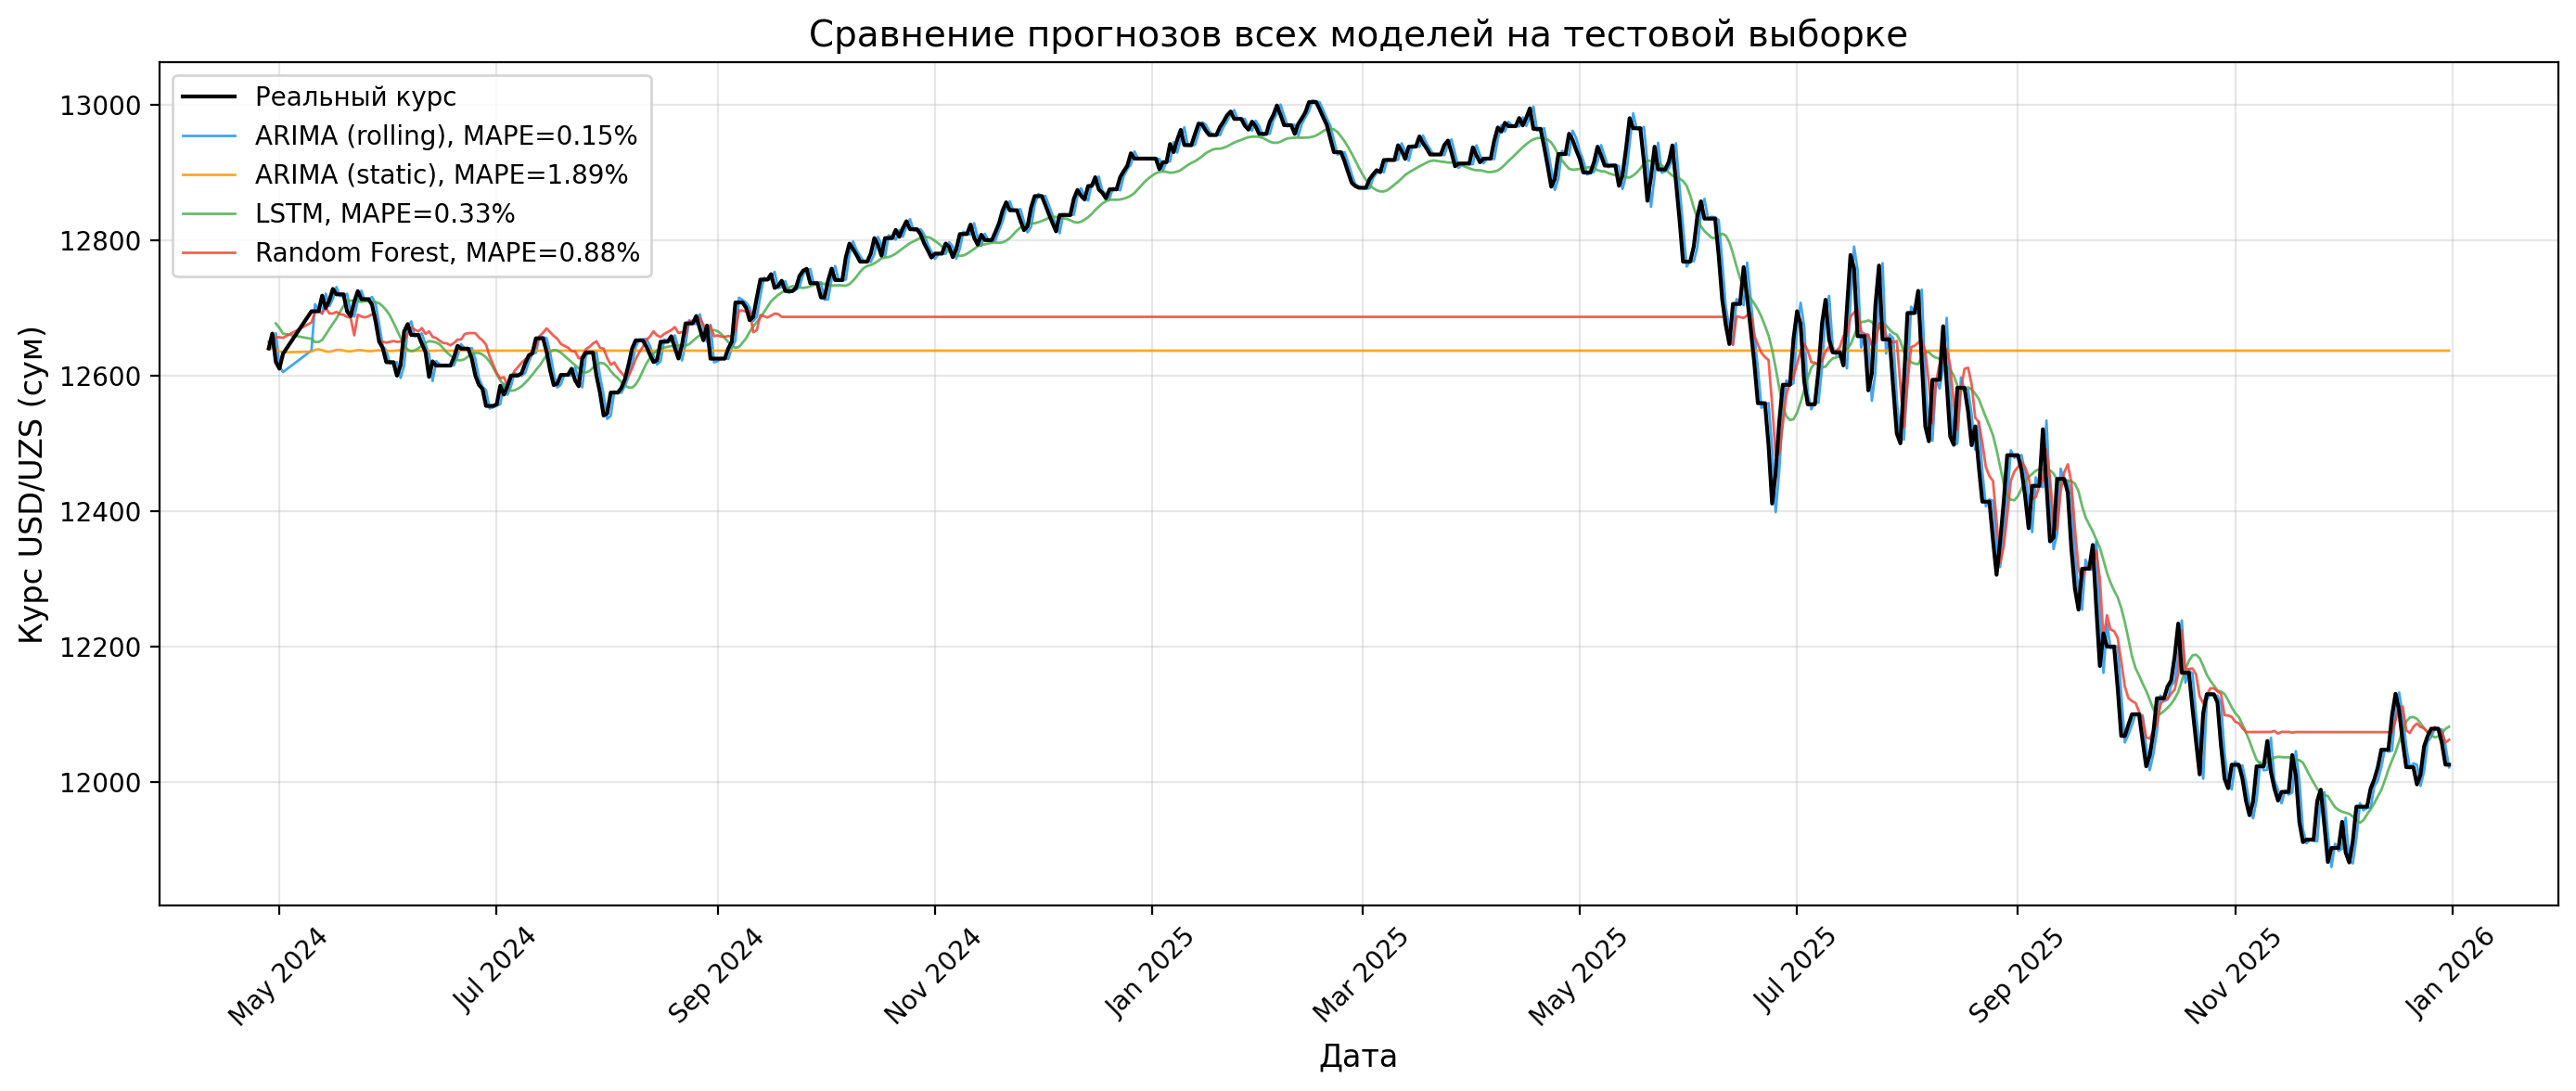
\includegraphics[width=\textwidth, height=0.78\textheight, keepaspectratio]{images/plot_all_models.png}
  \end{figure}
\begin{center}
  \vspace{-0.1cm}
  {\footnotesize
    \textcolor{primary}{\textbf{LSTM}} точнее всех без переобучения \quad|\quad
    \textcolor{orange}{\textbf{ARIMA static}} расходится с реальностью
  }

  \vspace{0.1cm}
  {\footnotesize
    \textcolor{blue}{\textbf{ARIMA rolling}} $\approx$ реальный курс
  }
\end{center}
\end{frame} % графики прогнозов всех моделей
\begin{frame}[shrink=10]{Графики прогнозов}
  \begin{columns}[T]
    \column{0.48\textwidth}
    \begin{center}
      \textbf{\color{primary}ARIMA (static)}\\[4pt]
      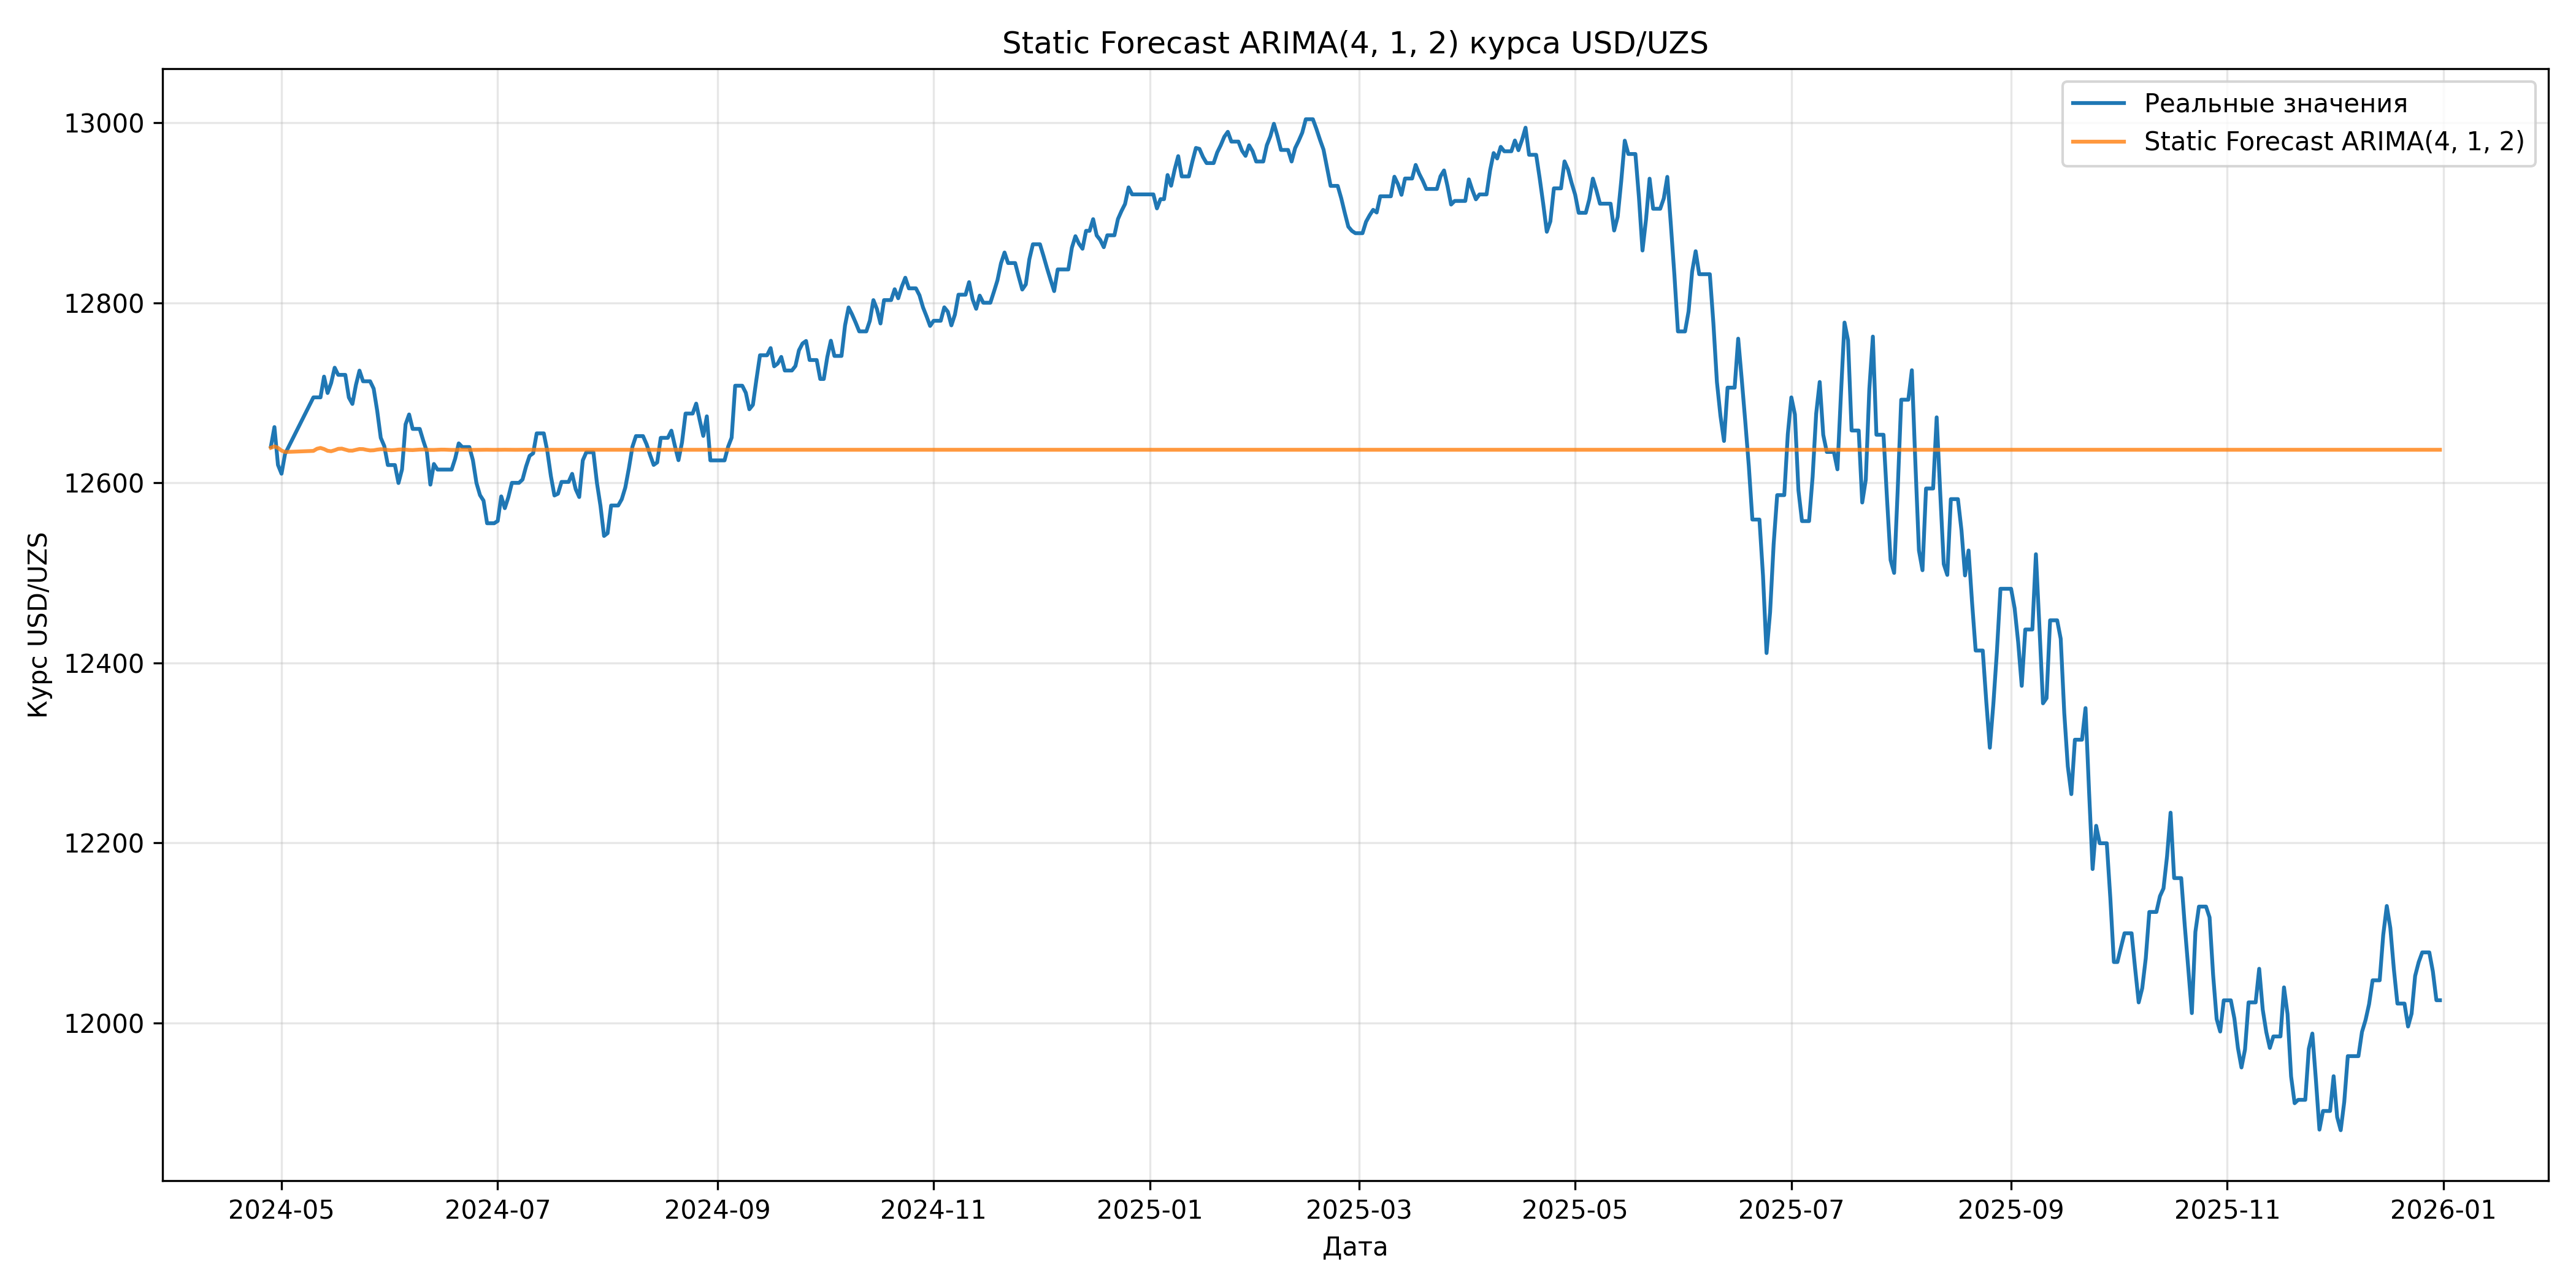
\includegraphics[width=\textwidth]{images/arima_static_forecast.png}
    \end{center}

    \column{0.48\textwidth}
    \begin{center}
      \textbf{\color{primary}LSTM}\\[4pt]
      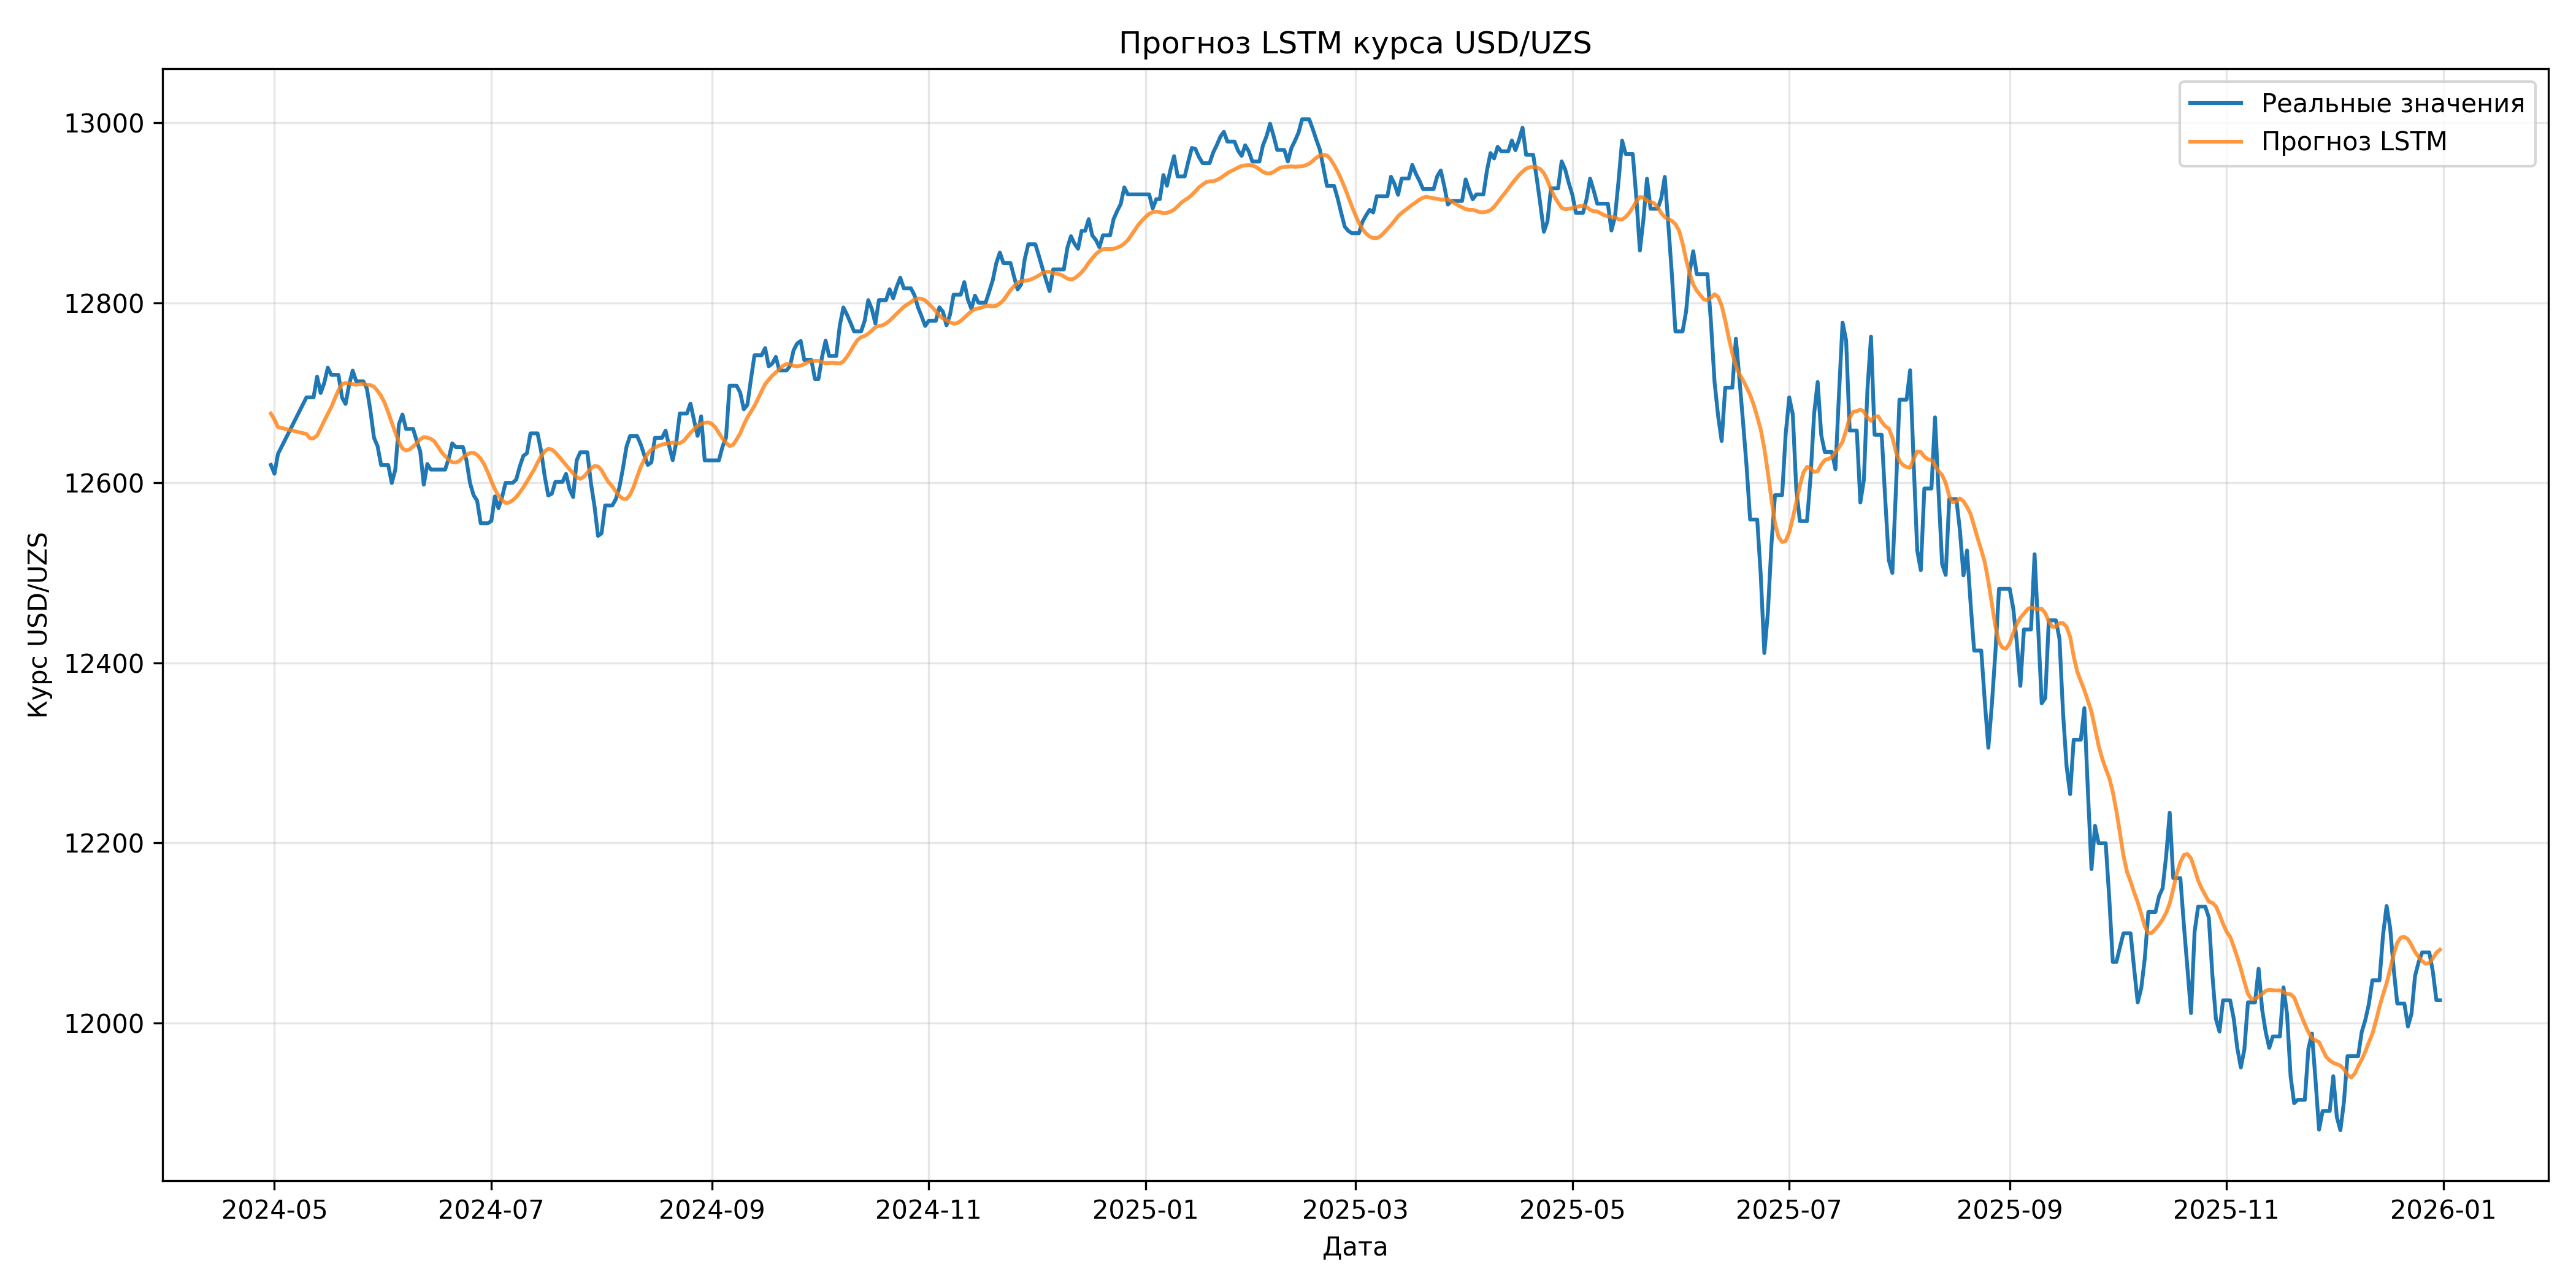
\includegraphics[width=\textwidth]{images/lstm_forecast.png}
    \end{center}
  \end{columns}

  \vspace{0.2cm}
  \begin{tcolorbox}[infobox]
    \small \textbf{Наблюдение:} LSTM точно следует за реальным курсом, тогда как статическая ARIMA сходится к линейному тренду.
  \end{tcolorbox}
\end{frame}          % графики прогнозов   % таблица результатов
% ─── Анализ ошибок по периодам (MAE по полугодиям) ─────────────────────────
\begin{frame}{Где модели ошибаются больше: MAE по полугодиям}

  \begin{columns}[T]
    % ─── Левая колонка: таблица ──────────────────────────────────────────
    \column{0.55\textwidth}
    \scriptsize
    \renewcommand{\arraystretch}{1.35}
    \setlength{\tabcolsep}{4pt}
    \begin{tabular}{>{\bfseries}lccccc}
      \toprule
      \textbf{Период} &
      \makecell{\textbf{ARIMA}\\\textbf{static}} &
      \textbf{RF} &
      \textbf{LSTM} &
      \makecell{\textbf{ARIMA}\\\textbf{roll.}} &
      \makecell{\textbf{Вол-}\\\textbf{ть}} \\
      \midrule
      1-е пг 2024$^{*}$ & 40  & 29  & 33 & 13 & 13,1 \\
      \rowcolor{light}
      2-е пг 2024       & 117 & 84  & 25 & 11 & 10,6 \\
      1-е пг 2025       & 268 & 220 & 37 & 16 & 15,4 \\
      \rowcolor{light}
      2-е пг 2025       & 382 & 59  & 62 & 32 & 32,2 \\
      \bottomrule
    \end{tabular}

    \vspace{0.25cm}
    {\tiny $^{*}$с апреля 2024 г.\quad MAE в сумах; «Вол-ть» --- средний модуль дневного изменения курса (сум/день).}

    % ─── Правая колонка: диаграмма ───────────────────────────────────────
    \column{0.45\textwidth}
    \centering
    \begin{tikzpicture}
      \begin{axis}[
        ybar, bar width=6pt,
        width=\textwidth, height=4.6cm,
        enlarge x limits=0.18,
        symbolic x coords={1п24, 2п24, 1п25, 2п25},
        xtick=data,
        x tick label style={font=\tiny},
        ylabel={MAE, сум}, ylabel style={font=\tiny},
        yticklabel style={font=\tiny}, ymin=0, ymax=420,
        legend style={font=\tiny, at={(0.5,1.12)}, anchor=south, legend columns=2, draw=none},
        nodes near coords, nodes near coords style={font=\tiny},
        every node near coord/.append style={anchor=south},
      ]
        \addplot[fill=danger!70, draw=danger]   coordinates {(1п24,40)(2п24,117)(1п25,268)(2п25,382)};
        \addplot[fill=success!70, draw=success] coordinates {(1п24,33)(2п24,25)(1п25,37)(2п25,62)};
        \legend{ARIMA static, LSTM}
      \end{axis}
    \end{tikzpicture}

    {\tiny\color{mygray}ARIMA static растёт с горизонтом, LSTM держит точность.}
  \end{columns}

  \vspace{0.2cm}
  \begin{tcolorbox}[infobox]
    \small \textbf{Вывод:} ошибки концентрируются в периоды повышенной волатильности. Модели со свежими данными (ARIMA rolling, RF) и нейросеть LSTM держат точность, тогда как статическая ARIMA деградирует с ростом горизонта прогноза (40\,$\to$\,382 сум).
  \end{tcolorbox}
\end{frame}
% ─── Rolling vs Static ARIMA ──────────────────────────────────────────────
\begin{frame}[shrink=10]{Почему ARIMA (rolling) обгоняет всех?}

  \begin{columns}[T]
    \column{0.48\textwidth}
    \begin{tcolorbox}[formulabox, title={\faSync\ Rolling Forecast}]
      \small
      На каждом шаге $t$:\\[3pt]
      \textcolor{accent}{\faAngleRight}~Добавляет \textbf{фактическое} $y_t$ в обучающую выборку\\[3pt]
      \textcolor{accent}{\faAngleRight}~Переобучает модель заново\\[3pt]
      \textcolor{accent}{\faAngleRight}~Прогнозирует $\hat{y}_{t+1}$\\[6pt]
      \textbf{Результат:} MAPE = \textcolor{success}{\textbf{0,15\%}}\\
      Модель всегда <<видит>> вчерашний курс
    \end{tcolorbox}

    \column{0.48\textwidth}
    \begin{tcolorbox}[warnbox]
      \small \textbf{\faLock\ Static (без переобучения)}\\[6pt]
      \textcolor{accent}{\faAngleRight}~Обучается \textbf{один раз} на train\\[3pt]
      \textcolor{accent}{\faAngleRight}~Прогнозирует весь test без обновления\\[3pt]
      \textcolor{accent}{\faAngleRight}~Прогноз сходится к линейному тренду\\[6pt]
      \textbf{Результат:} MAPE = \textcolor{danger}{\textbf{1,89\%}}\\
      В 12 раз хуже rolling
    \end{tcolorbox}
  \end{columns}

  \vspace{0.3cm}
  \begin{tcolorbox}[successbox]
    \small \textbf{Вывод:} ARIMA (rolling) побеждает \textit{не благодаря модели}, а благодаря \textbf{методологии переобучения}. При равных условиях (однократное обучение) \textbf{LSTM превосходит} и RF, и ARIMA --- MAPE 0,33\% vs 0,88\% и 1,89\%.
  \end{tcolorbox}
\end{frame}
% rolling vs static ARIMA
% ─── Ключевые выводы ─────────────────────────────────────────────────────
\begin{frame}[shrink=15]{Ключевые выводы}

  \begin{enumerate}\small
    \setlength\itemsep{0.15cm}

    \item \textbf{LSTM --- лидер при честном сравнении.} В условиях однократного обучения нейросеть LSTM (MAPE = 0,33\%) значительно превосходит Random Forest (0,88\%) и статическую ARIMA (1,89\%).

    \item \textbf{Rolling forecast --- мощный, но методологически особый.} ARIMA с rolling forecast (MAPE = 0,15\%) показывает наименьшие ошибки, однако это преимущество обусловлено постоянным переобучением, а не качеством самой модели.

    \item \textbf{Нейросети лучше улавливают нелинейность.} LSTM способна обучиться сложным паттернам валютного ряда, тогда как статическая ARIMA теряет точность уже на среднесрочном горизонте.

    \item \textbf{Random Forest уступает обоим подходам.} Несмотря на устойчивость к шуму, ансамблевый метод не смог эффективно моделировать автокорреляционную структуру ряда USD/UZS.

    \item \textbf{Практический вывод.} Для оперативного прогнозирования с обновлением данных оптимальна ARIMA (rolling). Для автономных прогнозов без переобучения --- LSTM.
  \end{enumerate}
\end{frame}
      % ключевые выводы
% ─── Финальный слайд «Спасибо за внимание» ────────────────────────────────
\begin{frame}[plain]
  \begin{tikzpicture}[remember picture, overlay]
    \fill[primary] (current page.north west) rectangle (current page.south east);
    \fill[accent] (current page.south west) rectangle
      ([yshift=6pt]current page.south east);
    \fill[white, opacity=0.05] ([xshift=-2cm,yshift=-2cm]current page.north east)
      circle (5cm);
  \end{tikzpicture}

  \begin{center}
    \vfill
    {\color{white}\fontsize{24}{28}\selectfont\bfseries Спасибо за внимание!}\\[0.5cm]
    {\color{accent}\rule{10cm}{1.5pt}}\\[0.5cm]
    {\color{white!80}\large Сравнение эффективности нейросетей и классических\\статистических моделей в прогнозировании курса валют}\\[0.3cm]
    {\color{white!60}\normalsize Автор | Группа}
    \vfill
    \begin{tcolorbox}[
      enhanced, boxrule=1pt, colframe=accent, colback=accent!20,
      width=10cm, center, rounded corners, left=10pt, right=10pt
    ]
      \color{darktext}\small
      \textbf{Главный вывод:}~При честном сравнении (однократное обучение) \textbf{LSTM} превосходит классические модели --- MAPE 0,33\% vs 0,88\% (RF) vs 1,89\% (ARIMA static)
    \end{tcolorbox}
    \vspace{0.5cm}
  \end{center}
\end{frame}
           % финальный слайд

\end{document}
